\documentclass[a4paper,10pt]{article}
\usepackage[cm]{fullpage}
\usepackage{tkz-orm}
\pagestyle{empty}
\usepackage{fancybox}
\usepackage[colorlinks=false,pdfborder={0 0 0}]{hyperref}

\def\myversion{0.1}
\def\mydate{2011-01-19}

\setlength{\parindent}{0in}

\begin{document}
\fancypage{\fbox}{}
\sffamily

\def\i#1{\textit{#1}}
\def\b#1{\textbf{#1}}

\tikzset{under/.style={label={[label distance=2mm,font=\itshape,align=center]below:#1}}}

% remember all nodes outside of external nodes
% \tikzstyle{every picture}+=[remember picture]

\begin{tikzpicture}
\node (title) {
  \begin{tabular}{c}
    \b{ORM2 Cheat sheet} \\
    Object Role Modeling \\
    version \myversion \\
    \mydate \\
    ~ \\
  \end{tabular}
};
\node [right=0 of title] {
\begin{tikzpicture}[orm]
\matrix[column sep=4mm,label={
  \b{n-ary predicates} are shown as sequence of \i{n} concatenated \b{role}
  boxes. Roles may have \b{role names}.}
]{
  \unary[label=above:died,under=unary]{}; &
  \binary[label=above:wrote,under=binary]{}; &
  \binary[label=above:\ormleft{written by},under={inverse\\reading}]{}; &
  \binary[label=above:owns/owned by,under={both\\readings}]{}; &
  \ternary[label=above:met \ldots at,under=ternary]{}; &
  \node{\i{\ldots}}; &
  \entity (p) {Person}; &
  \node[minimum width=10mm]{};
\\ };
\binary[right=of p,label=above:wrote] (w) {};
\plays (p) to (w);
\node[role name,below=of w.one north] {[author]};
\draw[color=white,line width=1mm,<->] (w.north east) to (w.south east);
\end{tikzpicture}
};
\end{tikzpicture}
%
\begin{tikzpicture}[orm]
\draw[dotted] (0,0) to (\linewidth,0);
\end{tikzpicture}
%
\begin{minipage}[t]{8cm}\vspace{0pt}%
\begin{tikzpicture}[orm]
\matrix[column sep=0mm,row sep=2.5mm,label={
Each role must be connected to exactely one \b{object type}.
}] {
  & \entity{A}; & \value{A}; & \\
\node[left]{\i{independent}}; &
  \entity{A$^!$}; & \value{A$^!$}; &
  \node[right]{can exist without playing roles}; \\
\node[left]{\i{duplicated}}; & 
  \entity[duplicated]{A}; & \value[duplicated]{A}; & 
  \node[right]{also elsewhere in model}; \\
\node[left]{\i{external}}; & 
  \entity[under=entity]{A\^{}}; & \value[under=value]{A\^{}}; & 
  \node[right]{details excluded from model}; \\
};
\end{tikzpicture}
\end{minipage}
\hfill
\begin{minipage}[t]{8.5cm}\vspace{0pt}%
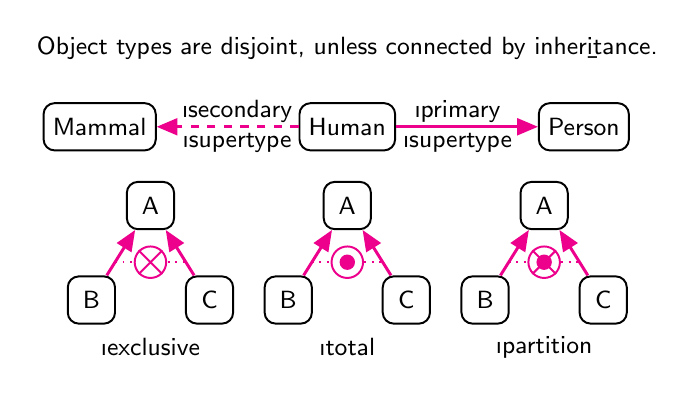
\begin{tikzpicture}[orm,level distance=12mm]
\node at (0,2)
  {Object types are disjoint, unless connected by \b{inheritance}.};

\entity (h) at (0,1) {Human};
\entity[right=18mm of h] (p) {Person};
\entity[left=18mm of h] (a) {Mammal};
\draw[suptype] (h) to (p);
\draw[supinterface] (h) to (a);
\node[align=left] at (-1.4,1.2) {\i{secondary}};
\node[align=left] at ( 1.4,1.2) {\i{primary}};
\node[align=left] at (-1.4,0.8) {\i{supertype}};
\node[align=left] at ( 1.4,0.8) {\i{supertype}};

\foreach \c/\x in {exclusive/-2.5,total/0,partition/2.5}{
  \entity (A) at (\x,0) {A} [edge from parent/.style=subtype]
    child {node [entity] (B) {B}} child {node [entity] (C) {C}};
  \limits ($(A)!.6!(B)$) to node[constraint=\c] {} ($(A)!.6!(C)$);
  \node at (\x,-1.8) {\i{\c}};
};
\end{tikzpicture}
\end{minipage}
%
\begin{tikzpicture}[orm]
\draw[dotted] (0,0) to (\linewidth,0);
\end{tikzpicture}
%
\begin{minipage}[t]{8cm}\vspace{0pt}%
\b{Uniqueness role constraints} span role combinations
with unique instances. Full predicates are always unique.
%
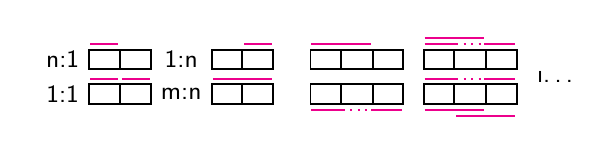
\begin{tikzpicture}[orm]
\matrix(m){
\node{n:1}; &
\binary[unique=1]{}; &
\node{1:n}; &
\binary[unique=2]{}; &
\node{~~~}; &
\ternary[unique=1-2]{}; &
\node{~}; &
\ternary[unique=1-3,skip unique=2,unique=1-2:2]{}; \\ 
\node{1:1}; &
\binary[unique=1,unique=2]{}; &
\node{m:n}; &
\binary[unique=1-2]{}; &
&
\ternary[unique=1-3:-1,skip unique=2:-1]{}; & 
&
\ternary[unique=1-3,skip unique=2,unique=1-2:-1,unique=2-3:-2]{}; 
\\
};
\node[right=0 of m] {\i{\ldots}};
\end{tikzpicture}
\end{minipage}
%
\hfill
%
\begin{minipage}[t]{8cm}\vspace{0pt}%
\b{Mandatory roles} as marked by a dot, must be played at least once. \ldots
\end{minipage}


\begin{tikzpicture}[orm]
\end{tikzpicture}

% TODO: 'external' constraints
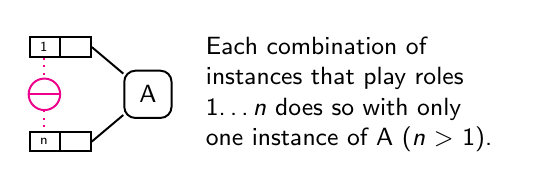
\begin{tikzpicture}[orm]
\entity(A){A};
\binary[left=of A,index=1,yshift=6mm](b){};
\binary[left=of A,index=n,yshift=-6mm](c){};
\plays (A) to (b.east) (A) to (c.east);
\limits (b.one south)to node[constraint=unique]{} (c.one north);
\node[right=3mm of A,text width=3.8cm]{Each combination of\\instances that
play roles 1\ldots \textit{n} does so with only one
instance of A (\textit{n} $>$ 1).};
\end{tikzpicture}

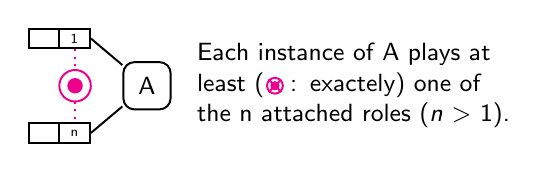
\begin{tikzpicture}[orm]
\entity(A){A};
\binary[left=of A,index=2:1,yshift=6mm](b){};
\binary[left=of A,index=2:n,yshift=-6mm](c){};
\plays (A) to (b.east) (A) to (c.east);
\limits (b.two south)to node[constraint=mandatory]{} (c.two north);
\node[right=2mm of A,text width=4cm]{Each instance of A plays at least
(~~~: exactely) one of the n attached roles (\textit{n} $>$ 1).};
\node[shape=partition,every constraint line,inner sep=0,minimum width=2mm,
  right=12mm of A] {};
\end{tikzpicture}


\begin{tikzpicture}[orm]
\draw[dotted] (0,0) to (\linewidth,0);
\end{tikzpicture}

% TODO: Reference modes ?

Not included yet constraints between roles: 
\b{exclusion}, \i{exclusive or}, \i{equality},
\i{subset/superset}, \i{equality}, \i{frequency}.
\b{ring constraints},
\b{value-comparision constraints}, \b{derived fact types},
\b{objectification}, object and role \b{value constraints}.
\b{deontic constraints}, \b{implied model parts}.

\begin{tikzpicture}[orm]
\draw[dotted] (0,0) to (\linewidth,0);
\end{tikzpicture}

This diagram has been created with tkz-orm (\url{http://purl.org/net/tkz-orm}).
Please note that some details are not fixed yet until the final release.

\end{document}
